\chapter{Conceptos básicos de ingeniería mecánica}

En este capítulo se especificarán los conceptos mínimos necesarios para la comprensión de los siguientes, tópicos que se suelen ver en los primeros años en un programa de ingeniería mecánica, por lo que puede ser obviado en caso de ya haber pasado por una formación similar. La descripción matemática y física de los fenómenos se entrega de manera simple para ejemplificar, evitando la complejidad de las expresiones más generales.

\section{Esfuerzo y deformación}

\subsection{Esfuerzo}

Uno de los principales intereses de la ingeniería mecánica es predecir, identificar y prevenir \textbf{mecanismos de falla} en componentes y sistemas. Entenderemos como la falla de un componente a un estado en el cual no puede cumplir con su \textbf{solicitud de carga o servicio} de acuerdo a diferentes perspectivas. Claramente, un componente fracturado (separado en dos partes) correspondería a una falla, sin embargo, también hablaremos de falla en otros casos en los que se comprometa funcionalidad o seguridad.

De la experiencia, sabemos que al aplicar una fuerza sobre un cuerpo este podría deformarse hasta romperse, sin embargo sabemos que existe una clara diferencia entre quebrar la rama de un árbol que el tronco entero, a pesar de estar constituidos del mismo material. Luego, es claro que la geometría juega un papel importante en la resistencia y debe ser normalizada para el análisis del \textbf{estrés mecánico}.

A este estrés lo llamaremos esfuerzo. Podemos expresar un tipo de esfuerzo $\sigma$, como por ejemplo el axial, de manera simple como:

\begin{equation}
    \sigma = \frac{F}{A}[Pa]
    \label{eq1}
\end{equation}

Con $F$ la fuerza (en $[N]$) aplicada sobre un cuerpo y $A$ (en $[m^{2}]$) la sección normal en la cual actúa esta fuerza. Esta medida da cuenta de la distribución de la fuerza sobre un área, y es una medida clave para el análisis mecánico de un cuerpo. 

Dadas las condiciones de un problema, el esfuerzo se comparará con diferentes valores, propios del material, impuestas como parámetro de diseño, o de las normas. A partir de tales métricas se podrá estimar si el componente cumple con la solicitación mecánica o falla.

De la experiencia de romper una rama, también sabemos que importa la forma en que actúa la fuerza, pues claramente es más sencillo romper la rama flectándola que tirándola. Así, el cálculo del esfuerzo dependerá de 3 factores clave: \textbf{Geometría}, \textbf{tipo de carga} y \textbf{condiciones de apoyo}. En la Figura \ref{fig:1} se ven los tipos de carga sobre un cuerpo. La \ref{eq1} corresponde a una condición de carga axial. 

\begin{figure}[h!]
    \centering
    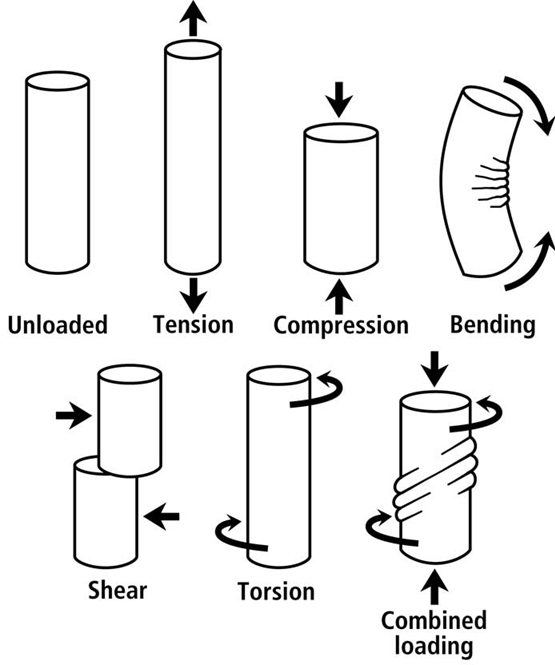
\includegraphics[width=0.5\linewidth]{imgs/loads.png}
    \caption{Tipos de carga: tensión (tracción), compresión, flexión, corte, torsión y carga combinada.}
    \label{fig:1}
\end{figure}

\subsection{Deformación}

Entenderemos como deformación al cambio geométrico de un cuerpo. Una forma de categorizar los tipos de deformación es respecto a la permanencia del cambio, donde si es reversible, se le llama \textbf{deformación elástica}, y en caso contrario, \textbf{deformación plástica}. La parte elástica es resultado de interacciones atómicas y/o moleculares (atracción, repulsión, desenrrollamiento de cadenas) con la fuerza aplicada, mientras que lo plástico está relacionado con el desplazamiento permanente de átomos o moléculas en la estructura. Por lo anterior, siempre existe deformación elástica antes de que se dé deformación plástica a medida que incrementa el esfuerzo.

En el caso de la deformación elástica, esta se suele modelar como una relación entre átomos contiguos mediante resortes a través de la Ley de Hooke. La fuerza correspondería entonces a:

\begin{equation}
    F=k\Delta l
\end{equation}

Donde $k$ es la constante elástica y $\Delta l$ el cambio de longitud respecto al largo inicial o natural $l_{0}$. En el caso de los materiales, esta ley se puede extender de manera simplista como:

\begin{equation}
    \sigma=E\varepsilon
\end{equation}

Donde $E$ es el \textbf{módulo de Young} o de elasticidad del material (en unidades de $[Pa]$) y $\varepsilon$ a la deformación (adimensional). De esta manera, un material con mayor $E$ será más \textbf{rígido}, es decir, con menor tendencia a deformarse. Una forma de representar a deformación $\varepsilon$ es la siguiente:

\begin{equation}
    \varepsilon = \frac{\Delta l}{l_{0}}=\frac{l_{f}-l_{0}}{l_{0}}
\end{equation}

Lo anterior es una aproximación lineal muy conveniente y que se sostiene en varios casos, sin embargo el comportamiento real de los materiales puede variar significativamente del régimen lineal. Para estos casos existen modelos más complejos con dependencias multivariable.

Los modelos para la deformación plástica tampoco son sencillos y quedan fuera del alcance de este apunte.

Las ecuaciones mostradas describen el caso ideal de deformación unidimensional, en el que un sólido se deforma exclusivamente a lo largo de un eje. La conservación de volumen implica que toda elongación longitudinal vaya acompañada de una contracción transversal (y viceversa), de modo que al estirar el material éste se estrecha en las direcciones perpendiculares. El \textbf{coeficiente de Poisson} $\nu$ cuantifica precisamente esta relación entre deformaciones longitudinal y transversal (adimensional). Sin embargo, ciertos materiales conocidos como \textbf{auxéticos} presentan un comportamiento opuesto: al someterse a tracción, también ensanchan su sección transversal, lo que se traduce en un valor negativo de $\nu$.

\subsection{Ensayo de tracción}

Una forma de caracterizar la relación esfuerzo-deformación es mediante el ensayo de tracción, como se observa en la Figura \ref{fig:2}. Como indica el nombre, una muestra de material con forma determinada es traccionado hasta la fractura, midiendo la fuerza y el desplazamiento de las mordazas que ejercen la fuerza, con cierto ajuste, o directamente a través de un extensómetro. Estos datos luego son transformados a su equivalente en esfuerzo y deformación, logrando las curvas observadas. 

\begin{figure}[h!]
    \centering
    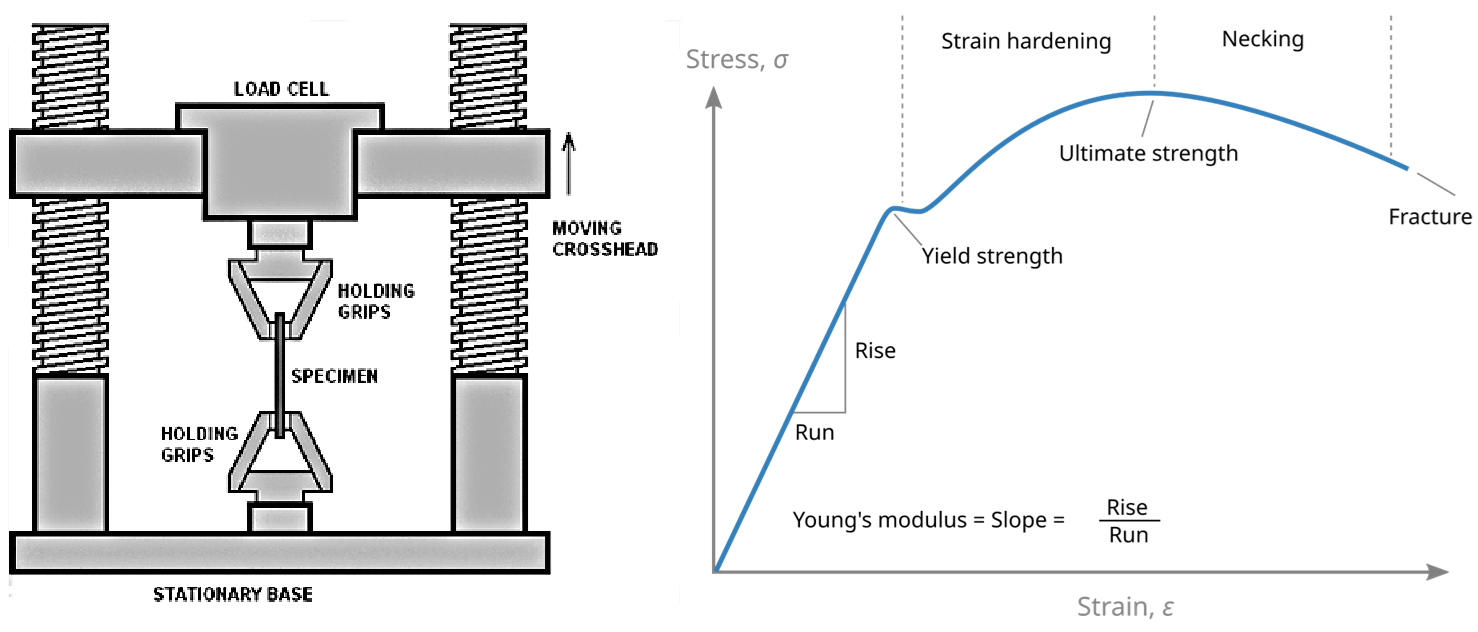
\includegraphics[width=0.92\linewidth]{imgs/es1.png}
    \caption{Ensayo de tracción, a la izquierda, montaje, a la derecha, curva de esfuerzo-deformación.}
    \label{fig:2}
\end{figure}

Para el material exhibido en la Figura \ref{fig:2}, se observa una región inicial lineal, la cual corresponderá a la parte elástica. Al límite de esta región se le conoce como \textbf{esfuerzo de fluencia} o límite elástico (yield strength), simbolizado como $\sigma_{y}$, y es una \textbf{propiedad mecánica} de los materiales. La pendiente es entonces el módulo de Young $E$.

De la misma manera, al esfuerzo máximo en la curva le llamaremos \textbf{resistencia última a la tracción} $\sigma_{UTS}$ (ultimate strength). Más allá de este punto, se da un modo de deformación local conocido como \textbf{estrangulamiento} o \textit{necking} hasta la fractura del espécimen. Si bien, se observa que el esfuerzo baja en la curva, esto es así porque para el cálculo se considera el área inicial $A_{0}$ en lugar de la real. Con tal corrección, se observaría que el esfuerzo sigue aumentando.

La forma de esta curva no es igual para cada tipo de material, y también existen variaciones dentro de las mismas familias. En la Figura \ref{fig:3} se observan curvas representativas de cada tipo de material. De aquí se podría inferir, por ejemplo que en general los cerámicos son los materiales más rígidos y presentan un comportamiento elástico bastante lineal, mientras que los polímeros serían los menos resistentes. Entraremos en detalle respecto a los valores y comparaciones entre materiales en los próximos capítulos.

\begin{figure}[h!]
    \centering
    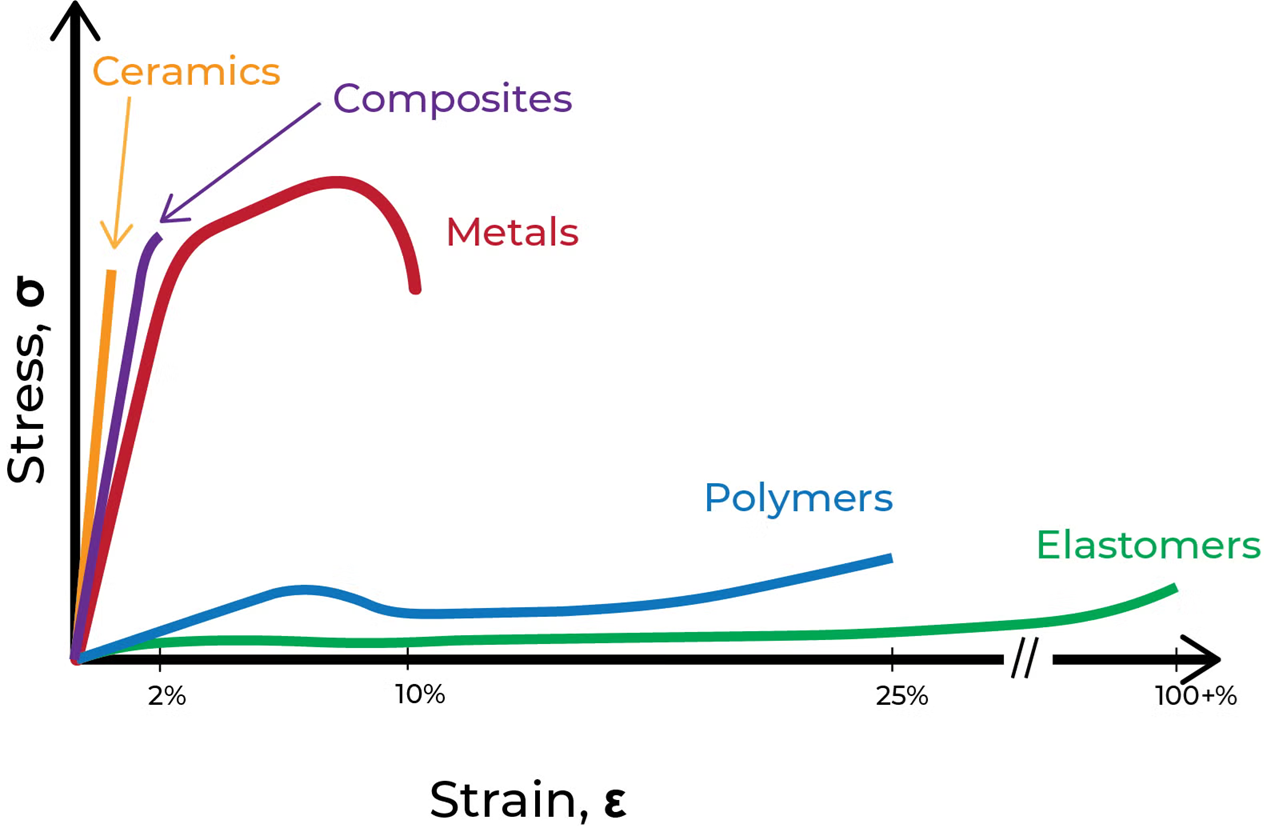
\includegraphics[width=0.75\linewidth]{imgs/tract.png}
    \caption{Ensayos de tracción para distintos tipos de materiales.}
    \label{fig:3}
\end{figure}

La \textbf{elongación final} $\varepsilon_{f}$ es la deformación alcanzada por la muestra hasta la falla. Es una propiedad mecánica que da cuenta de la ductilidad del material.

\section{Falla de componentes}

Como se mencionó anteriormente, a través del cálculo del estado de esfuerzos y diferentes métricas se podrá ajustar correctamente el diseño y la selección de materiales para prevenir fallas. Por ejemplo, si la deformación elástica es admisible, pero no así la plástica, un criterio sería simplemente:

\begin{equation}
    \sigma < \sigma_{y}
\end{equation}

Luego, se buscará un material con un $\sigma_{y}$ adecuado tal que cumpla la relación, o bien, se harán modificaciones en el diseño para disminuir el esfuerzo resultante. 

Considerando que estos modelos físicos surgen de aproximaciones y simplificaciones a la realidad, existe incerteza respecto a la exactitud de estos cálculos, por esto, se suele utilizar un \textbf{factor de seguridad} $f_{s}>1$ para garantizar seguridad en el servicio del componente, de la forma:

\begin{equation}
   \frac{\sigma_{y}}{\sigma} = f_{s}>1.0
\end{equation}

Esto aumenta la solicitud al material. La magnitud de este factor dependerá de normas y de la certeza en los cálculos empleados, intentando mantener el valor lo más reducido posible, pues su consecuencia podría implicar un sobredimensionamiento costoso del componente o sistema.

Una restricción sobre el diseño que podría ser más fuerte es limitar la deformación. Para aplicaciones de precisión o de tolerancias ajustadas, una deformación pequeña puede generar contactos indeseados entre componentes o modificar la trayectoria de otros.

Los criterios ejemplificados anteriormente son estáticos, es decir, no consideran fenómenos asociados al daño acumulado con el avance del tiempo.

Una de estas formas de daño acumulado es la \textbf{fatiga}, y está relacionada con el crecimiento de grietas o defectos en la estructura del material hasta generar una fractura (Figura \ref{crack}). Una \textbf{grieta} es una discontinuidad que no permite la distribución uniforme del esfuerzo, sino que lo concentra en su reducida geometría local, fracturando secuencialmente el material.

\begin{figure}[h!]
    \centering
    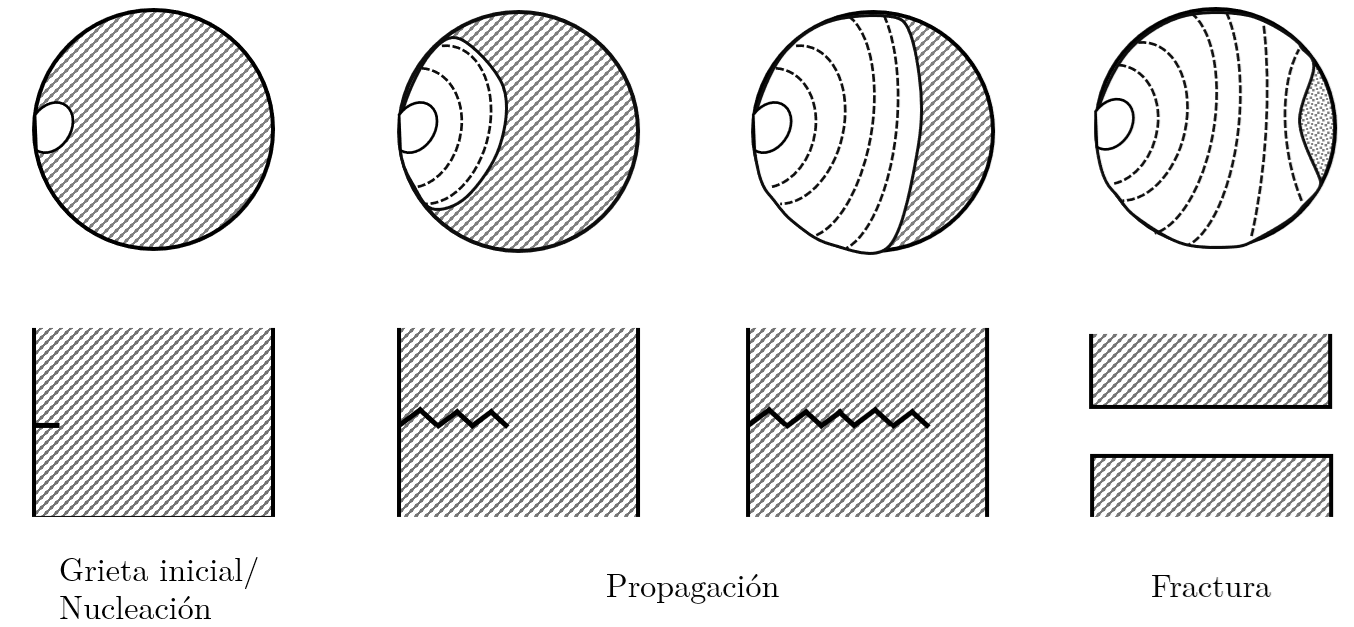
\includegraphics[width=0.9\linewidth]{imgs/crack.png}
    \caption{Mecanismo de crecimiento de grieta por fatiga. (1) Nucleación o iniciación, (2) Propagación, (3) Fractura, se observa una sección de la superficie rugosa y cristalina (crecimiento rápido de grieta, frágil), y otra suave y brillante (crecimiento lento).}
    \label{crack}
\end{figure}

Este crecimiento de grieta a través de la fatiga está relacionado con cargas cíclicas y debilita al material, reduciendo su vida útil a pesar de que los esfuerzos no sean superiores a $\sigma_{y}$. El daño inducido por estas cargas depende de múltiples variables, por ejemplo:

\begin{itemize}
    \item Propiedades intrínsecas del material.
    \item Carga: Tipo, amplitud, media, y en menor medida, frecuencia.
    \item Geometría: Tamaño de la pieza, concentradores de esfuerzo, defectos.
    \item Calidad de la superficie: Tratamiento, grietas.
    \item Condiciones ambientales: Humedad, temperatura, agentes químicos.
\end{itemize}

La fatiga como parámetro de diseño permite calcular la vida útil del material, mediante el uso de la curva de vida amplitud-ciclos o diagrama de Wöhler (Figura \ref{fig:4}).

\begin{figure}[h!]
    \centering
    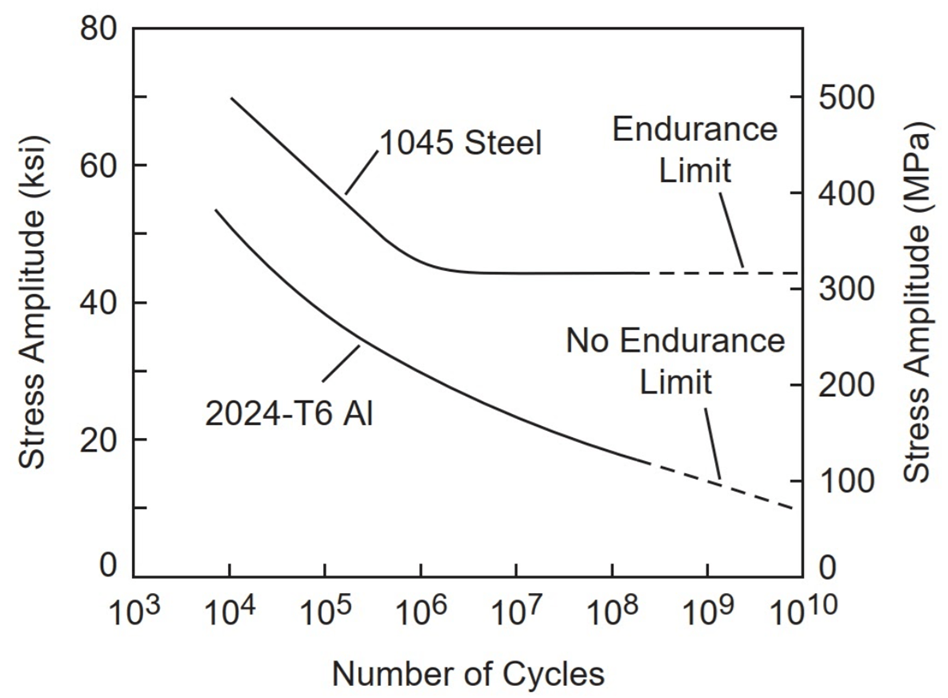
\includegraphics[width=0.7\linewidth]{imgs/sn.png}
    \caption{Curva de Wöhler para aleación de aluminio y acero.}
    \label{fig:4}
\end{figure}

En el ejemplo se observan 2 aleaciones metálicas ampliamente estudiadas. Nótese el \textit{endurance limit} (límite de fatiga), el cual indica que para amplitudes inferiores a este el material tiene vida infinita.

Dado que esto depende en parte de un tamaño de grieta, el material también podría fallar de manera estática si es que posee una grieta inicial. Esta grieta avanzaría de forma rápida e inestable hasta la ruptura, sin necesidad de ciclos de carga en función de la \textbf{resistencia a la propagación de grietas} del material.

El parámetro $K_{IC}$, determinado mediante ensayos cuantifica la resistencia intrínseca del material al crecimiento de grietas (bajo ciertas condiciones específicas, como régimen elástico) y resulta fundamental para diseñar y evaluar componentes con concentradores de esfuerzo, pues define el umbral crítico que evita fallas frágiles. Una forma de usar este parámetro comparándolo con el factor de intensidad de la grieta $K$ $([Mpa\sqrt{m}]$): 

\begin{equation}
    K=\beta \sigma\sqrt{a\pi} < K_{IC} \implies \text{No hay fractura rápida}
\end{equation}

Con $\beta$ un parámetro geométrico y $a$ el tamaño de la grieta. Si bien, esta medida podría dar cuenta de la \textbf{tenacidad} del material, la energía absorbida antes de la fractura (Figura \ref{fig:5}), existen otros ensayos y medidas más directas que consideran además la deformación plástica, como el ensayo de impacto de Charpy o Izod. Los materiales frágiles suelen presentar deformación plástica despreciable (como se observa en la Figura \ref{fig:5}) y alta sensibilidad a concentradores de esfuerzo, como sucede con vidrios y cerámicos.

\begin{figure}[h!]
    \centering
    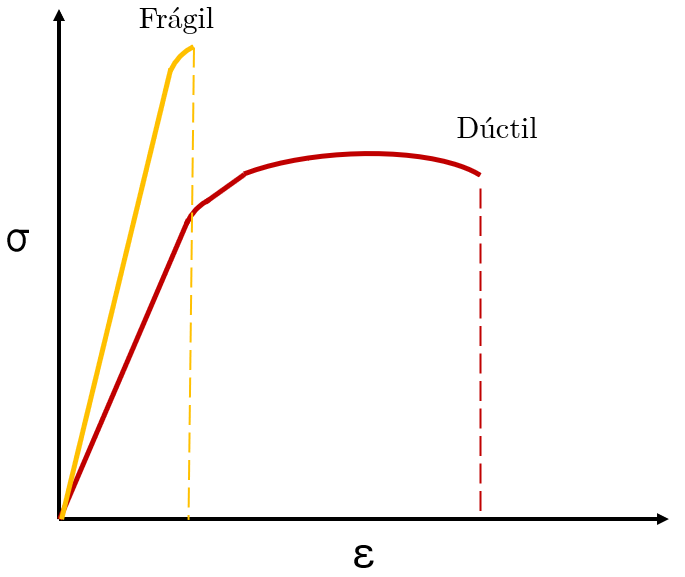
\includegraphics[width=0.55\linewidth]{imgs/tough.png}
    \caption{Curva de esfuerzo deformación para un material dúctil (alta deformación plástica) y uno frágil.}
    \label{fig:5}
\end{figure}

Otra causa para la falla de materiales es la \textbf{termofluencia} o \textbf{creep}, que corresponde a deformación progresiva y dependiente del tiempo que sufre un material bajo carga constante a temperaturas elevadas, que puede culminar en falla sin necesidad de aumentar la tensión aplicada. 

\section{Dureza}

La dureza es una propiedad mecánica de los materiales que mide la capacidad de resistir la penetración o deformación plástica localizada en su superficie bajo una carga concentrada (Figura \ref{dur}). Se determina mediante ensayos de indentación (Brinell, Rockwell, Vickers, Shore, entre otros) que cuantifican el tamaño de la huella dejada por un indentor bajo una carga controlada. Como propiedad mecánica complementaria a la resistencia a la tracción, la dureza ofrece una medida rápida y casi no destructiva de la resistencia al desgaste y a la abrasión.

\begin{figure}[h!]
    \centering
    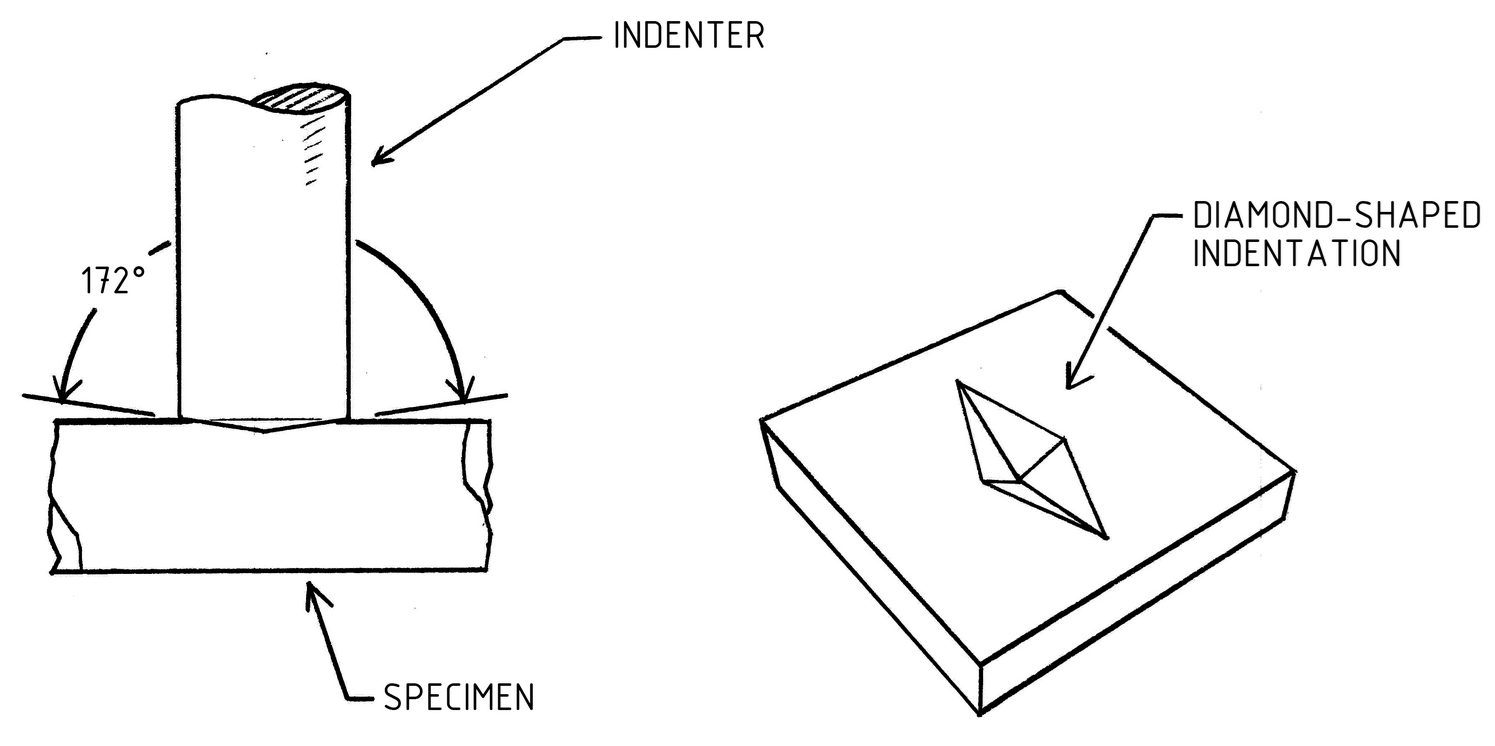
\includegraphics[width=0.7\linewidth]{imgs/indent.png}
    \caption{Ensayo de dureza, existen diversas variantes, pero esencialmente se indenta una muestra y se mide la huella.}
    \label{dur}
\end{figure}

Así, en la interacción mecánica entre dos materiales de diferente dureza, el más blando es más susceptible a deformarse y ceder, mientras que el más duro actúa como agente agresor y conserva su forma. Esta diferencia de dureza determinará el mecanismo de desgaste (abrasión, adhesión, fatiga de contacto) que primará en la interacción, así como la tasa de desgaste.

Un material de alta dureza evita la deformación plástica localizada y la concentración de tensiones que dan origen a grietas, prolongando la vida útil del componente. Además, su superficie lisa y resistente dificulta la penetración y el arranque de material bajo cargas de deslizamiento, reduciendo el desgaste por fricción, luego, estos materiales son ideales para soportar cargas deslizantes en transmisión o para aplicaciones con impactos frecuentes.

Por otro lado, un material frágil presenta baja tenacidad y prácticamente nula ductilidad, de modo que se fractura de forma repentina al superar su límite elástico. Esto conlleva fallos catastróficos sin señal previa, mala absorción de energía ante impactos o vibraciones y alta susceptibilidad a la propagación de grietas, lo que limita su uso en aplicaciones donde la seguridad y la fiabilidad sean críticas.

Dado que estos fenómenos se presentan principalmente en la superficie de un material, se han desarrollado técnicas o \textbf{tratamientos de endurecimiento superficial} que generan una capa externa de elevada dureza y resistencia al desgaste, mientras el núcleo conserva la ductilidad y tenacidad necesarias, optimizando así la durabilidad y seguridad de la pieza.

\section{Transferencia de calor}

Se define la temperatura como una magnitud física intensiva, proporcional a la energía cinética media de las partículas que constituyen un sistema termodinámico. Cuando dos cuerpos a distinta temperatura entran en contacto, se genera un flujo de energía térmica entre ellos, denominado transferencia de calor, que persiste hasta alcanzar el equilibrio térmico. La transferencia de calor se da a través de 3 mecanismos (Figura \ref{calors}):

\begin{itemize}
  \item Conducción: transferencia de energía mediante colisiones entre partículas adyacentes en un material sólido o estacionario.
  \item Convección: transporte de calor por el movimiento de un fluido (líquido o gas), ya sea natural o forzado.
  \item Radiación: emisión y absorción de energía en forma de ondas electromagnéticas, que puede ocurrir incluso en el vacío.
\end{itemize}

Los fenómenos de transferencia térmica están determinados por las propiedades termofísicas de los materiales. Cuando un flujo de calor atraviesa un sólido, la variación de su temperatura viene definida por:

\begin{itemize}
  \item Densidad, \(\rho\) [kg/m³], masa por unidad de volumen.
  \item Calor específico, \(c_p\) [J/(kg\,K)], energía necesaria para elevar 1 K la temperatura de 1 kg.
  \item Conductividad térmica, \(k\) [W/(m\,K)], capacidad de transmitir flujo de calor por unidad de gradiente de temperatura.
\end{itemize}

\begin{figure}[h!]
    \centering
    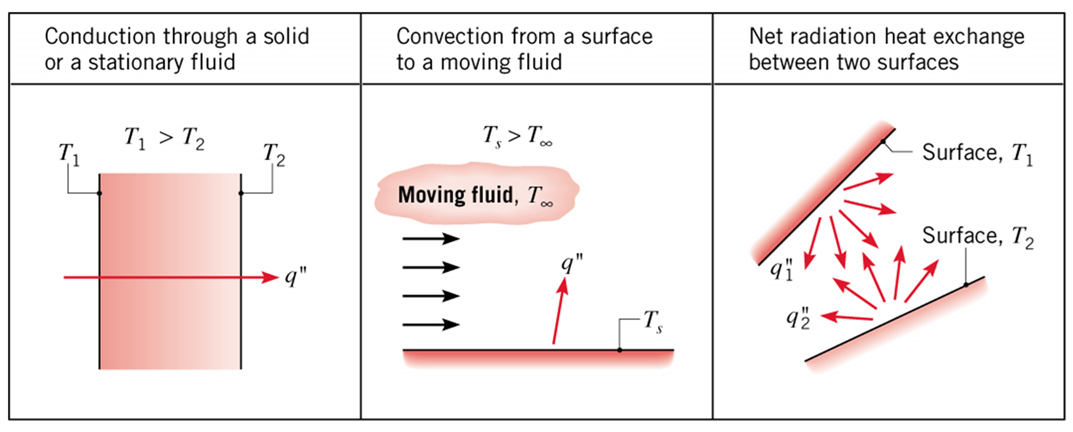
\includegraphics[width=0.85\linewidth]{imgs/calor.png}
    \caption{Mecanismos de transferencia de calor.}
    \label{calors}
\end{figure}

La difusividad térmica, \(\alpha\), sintetiza estas tres magnitudes y mide la rapidez con que se propaga una perturbación térmica:

\begin{equation}
  \alpha = \frac{k}{\rho\,c_p}
  \quad [\mathrm{m^2/s}]
\end{equation}

En la práctica todos los materiales exhiben alguna dependencia de sus propiedades mecánicas con la temperatura. No obstante, hay magnitudes que muestran variaciones muy pequeñas y a menudo se tratan como constantes en ciertas aplicaciones. En la Figura \ref{fig:ttt} se observa una variación leve del módulo de Young para dos aleaciones de acero en un rango amplio de temperaturas, mientras que el límite elástico presenta una variación más severa.

\begin{figure}[h!]
    \centering
    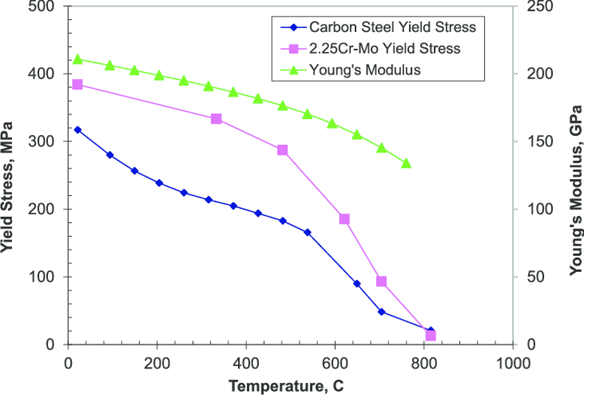
\includegraphics[width=0.7\linewidth]{imgs/tempgraf.png}
    \caption{Variación del módulo de Young y el límite elástico para dos aleaciones de acero.}
    \label{fig:ttt}
\end{figure}

Un fenómeno relevante ligado al cambio de temperatura es la \textbf{dilatación térmica} $\beta$. El aumento de la energía cinética de las partículas desplaza su distancia de equilibrio, alejándolas. Como consecuencia, el cuerpo presentará un aumento de volumen que dependerá del parámetro $\beta$, o reducción en caso de que la temperatura descienda.

La dilatación térmica en sistemas mecánicos puede alterar significativamente la holgura entre dos componentes. Si existe movimiento relativo, surgirán fuerzas de rozamiento y abrasión en caso de contacto; y si la expansión está impedida, se generan presiones internas que originan un \textbf{esfuerzo térmico}.

\section{Materiales de ingeniería}

\subsection{Clasificación}

Un material de ingeniería es aquel cuya composición y estructura se controlan deliberadamente durante su fabricación, siguiendo métodos y pruebas estandarizadas para que sus propiedades (mecánicas, térmicas, eléctricas o químicas) sean siempre las mismas (dentro de cierto rango). De esta forma, permiten diseñar piezas y estructuras con certeza respecto a su comportamiento y desempeño.

Estos materiales se suelen agrupar en 4 familias en función del \textbf{enlace químico} predominante en su estructura (Figura \ref{bons}), pues esto determinará en gran medida las propiedades mecánicas, térmicas y eléctricas:

\begin{figure}[h!]
    \centering
    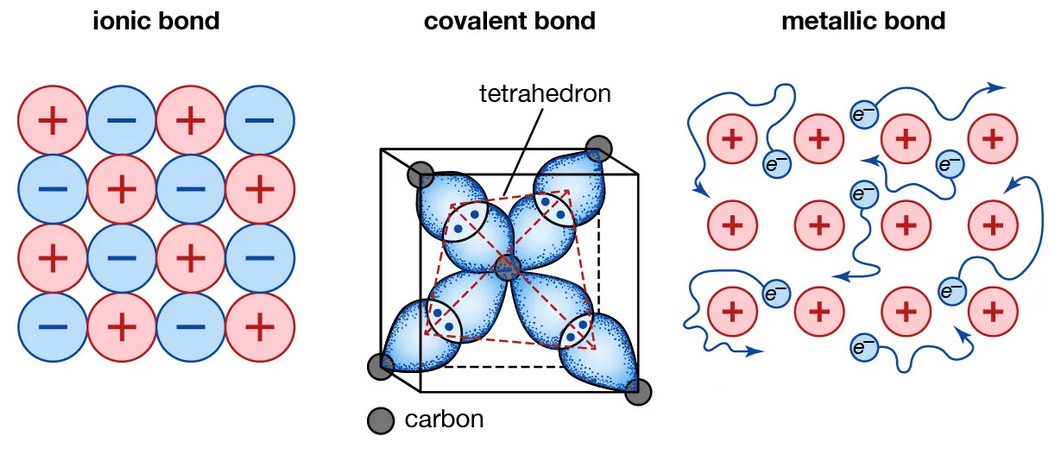
\includegraphics[width=0.75\linewidth]{imgs/bonds.png}
    \caption{Tipos de enlaces atómicos en materiales de ingeniería.}
    \label{bons}
\end{figure}

\textbf{Materiales metálicos}
    \begin{itemize}
      \item Enlace metálico con electrones libres.
      \item Alta conductividad térmica y eléctrica.
      \item Excelente ductilidad, maleabilidad y tenacidad.
      \item Buena resistencia mecánica y capacidad de deformación plástica.
    \end{itemize}

\textbf{Materiales cerámicos}
  
    \begin{itemize}
      \item Enlaces iónicos y/o covalentes muy fuertes.
      \item Elevada dureza y estabilidad a altas temperaturas.
      \item Baja tenacidad: comportamiento frágil ante impactos.
      \item Aislantes eléctricos y térmicos.
    \end{itemize}

\textbf{Materiales poliméricos}
  
    \begin{itemize}
      \item Cadenas moleculares unidas por enlaces covalentes.
      \item Baja densidad y buen aislamiento térmico y eléctrico.
      \item Amplia variedad de rigidez y elasticidad (termoplásticos, termofijos, elastómeros).
      \item Resistencia química y facilidad de procesado.
    \end{itemize}

\textbf{Materiales compuestos}
  
    \begin{itemize}
      \item Matriz (polímero, metal o cerámico) reforzada con fibras o partículas.
      \item Elevada resistencia específica.
      \item Propiedades a medida según combinación de componentes.
      \item Versatilidad en forma y aplicación, adaptables a exigencias de diseño.
    \end{itemize}

Esta clasificación y las propiedades comunes de cada familia simplifican la selección inicial de materiales para las condiciones operativas. Sin embargo, los \textbf{parámetros de diseño} (restricciones y objetivos que guían el proceso) determinan la idoneidad final de la elección. Por ejemplo, si se necesita una pieza rígida y resistente a la corrosión, un cerámico podría parecer la opción ideal; no obstante, podría resultar incompatible con los procesos de manufactura habituales o disponibles. De esta manera, la selección del material va a seguir los siguientes criterios:

\begin{itemize}
    \item Rendimiento mecánico (resistencia, dureza, tenacidad).
    \item Condiciones de servicio (temperatura, ambiente químico, cargas cíclicas).
    \item Factores económicos (coste de materia prima, procesamiento y reciclado).
    \item  Sostenibilidad y ciclo de vida (reutilización, huella ambiental).
    \item Disponibilidad y normativas (certificaciones, estandarización internacional).
\end{itemize}

Dada la composición química y el tipo de enlace, el material adquiere una \textbf{microestructura} que describe cómo se agrupan sus átomos. Si ese agrupamiento presenta un orden periódico a largo alcance, hablamos de una \textbf{red cristalina}; en caso contrario, la estructura es \textbf{amorfa} (Figura \ref{cris}). En un sólido cristalino, esos arreglos atómicos ordenados se extienden más allá de la escala atómica para formar \textbf{granos} distinguibles (Figura \ref{mic}), dentro de los cuales todos los cristales comparten una misma orientación. Esta organización, sea en forma de granos o de red desordenada, condiciona de manera decisiva las propiedades mecánicas, térmicas y eléctricas del material.

\begin{figure}[h!]
    \centering
    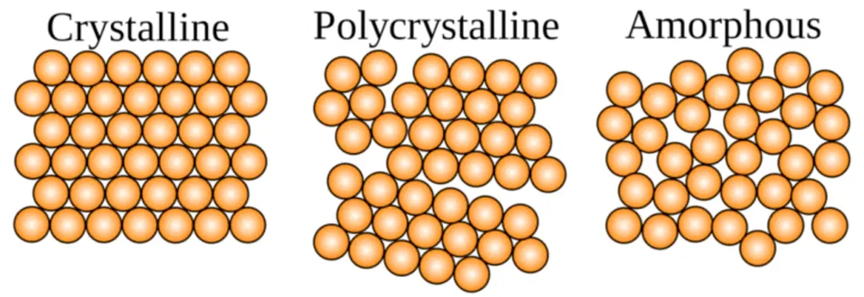
\includegraphics[width=0.9\linewidth]{imgs/crist.png}
    \caption{Esquema de microestructuras: Monocristal, policristal (varias orientaciones) y amorfo.}
    \label{cris}
\end{figure}

Es posible controlar la microestructura del material actuando en cada etapa del ciclo de vida: durante su formación inicial, en el procesamiento de la materia prima y a través de tratamientos posteriores. Al ajustar las diferentes variables, podemos diseñar arreglos atómicos y granulometrías que optimicen las propiedades finales del material para algún servicio específico. Eventualmente, durante el servicio, las condiciones podrían modificar o dañar la microestructura del material, iniciando mecanismos de falla.

\begin{figure}[h!]
    \centering
    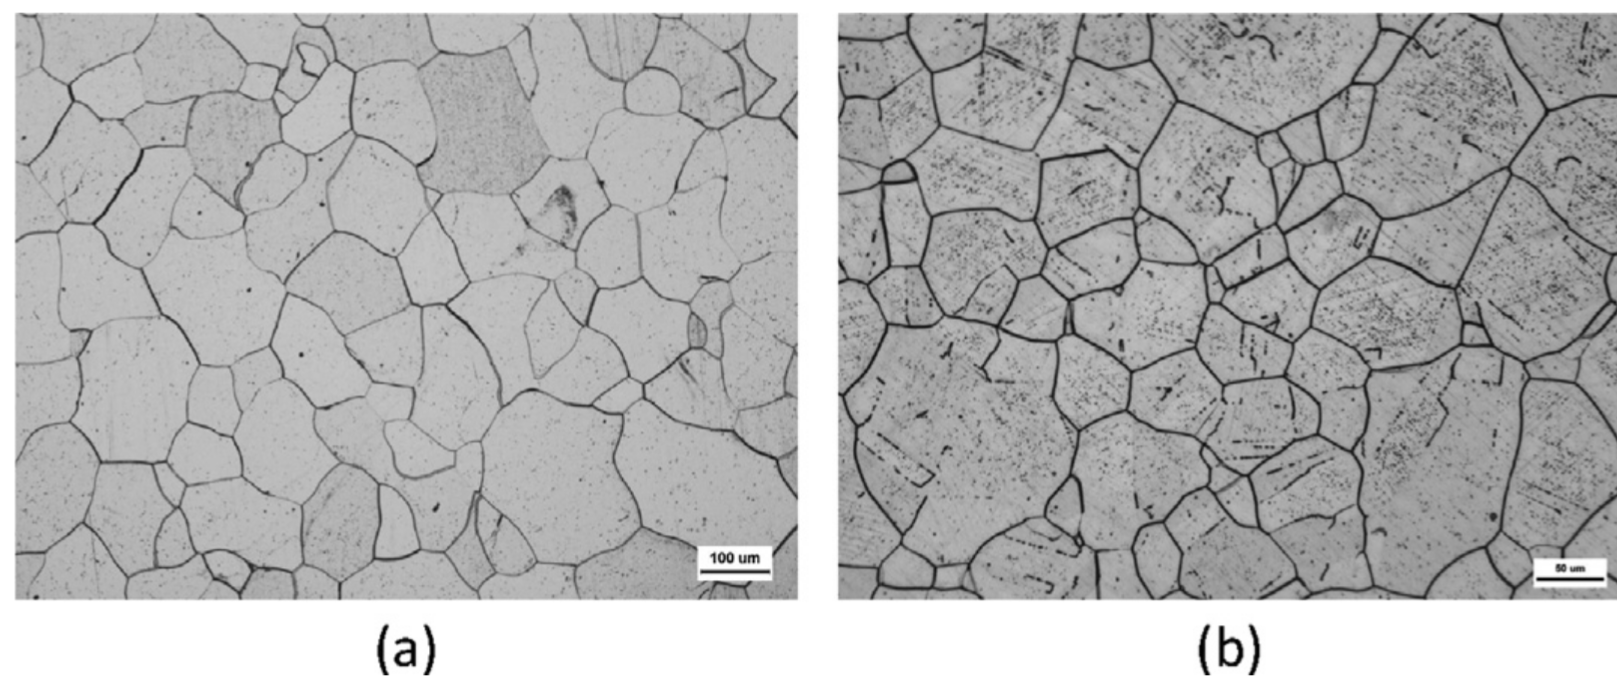
\includegraphics[width=0.9\linewidth]{imgs/micr.png}
    \caption{Fotografía de granos en un material a través de microscopio.}
    \label{mic}
\end{figure}

\subsection{Materiales y valores típicos}

Como vimos anteriormente, las distintas familias de materiales exhiben rangos característicos de propiedades, pero la elección de un material implica evaluar múltiples criterios de diseño. Para simplificar este proceso, resulta muy útil representar gráficamente las variables clave. En la Figura \ref{props}, por ejemplo, los materiales se sitúan según su rigidez y densidad; así, al fijar una rigidez objetivo, podemos identificar de inmediato la opción más ligera que la cumpla.

\begin{figure}[h!]
    \centering
    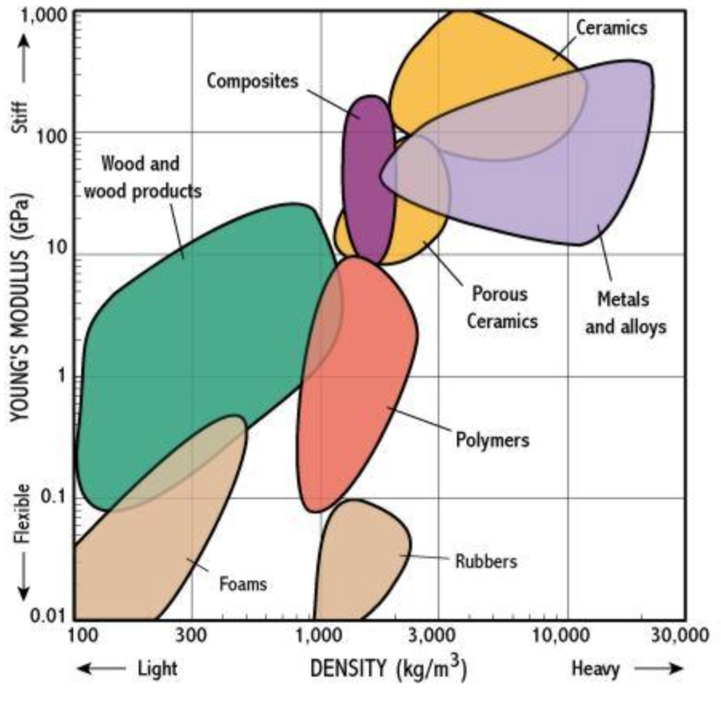
\includegraphics[width=0.6\linewidth]{imgs/comp.png}
    \caption{Gráfico rigidez-densidad para materiales de ingeniería, útil para optimizar la resistencia a la deformación/peso.}
    \label{props}
\end{figure}

Actualmente, este tipo de mapas se da en aplicaciones computacionales interactivas, las cuales permiten hacer el cruce de parámetros y agilizar la selección del material, así como otorgar información relevante respecto a los costos, aplicaciones típicas, procesos de conformado, etc. De esta manera, la labor de ingeniería no es solo identificar el material que cumple con las exigencias mecánicas, sino que además optimizar el desempeño, la economía y la sostenibilidad del diseño en estudio.

En la formación de ingeniería mecánica y metalúrgica se presta especial atención a los materiales de uso industrial más extendido. El acero ocupa un lugar central: una \textbf{aleación} (mezcla de elementos en la que al menos uno es metálico) de hierro y carbono. Las variaciones en su composición (contenido de carbono y elementos de aleación) y en los \textbf{procesos de fabricación} (laminado, forja, extrusión, tratamientos térmicos) definen la microestructura resultante y, con ello, sus propiedades mecánicas. Otras aleaciones estudiadas son las de aluminio (aluminio combinado con cobre), bronce (cobre y estaño), y latón (cobre y zinc).

\begin{table}[htbp]
  \centering
  \small
  \caption{Composición y costo de familias de materiales}
  \label{tab:prop_mat_comp_costo}
  \begin{tabular}{@{} l l c @{}}
    \toprule
    Material                  & Composición                          & Costo (\$/kg) \\
    \midrule
    Aceros al carbono         & Fe + 0.05–1.2\% C                    & 0.8–1.2       \\
    Aceros de aleación        & Fe + C + 2–8\% (Cr, Ni, Mo, V…)      & 1.0–1.5       \\
    Aleaciones de aluminio    & Al + (Si, Mg, Cu, Zn)                & 1.5–3.0       \\
    Aleaciones de titanio     & Ti + (Al, V)                         & 20–30         \\
    Superaleaciones de níquel & Ni + Cr, Co, Al, Ti…                 & 50–80         \\
    Cobre puro                & Cu                                   & 5.0–7.0       \\
    Bronce                    & Cu + 5–12\% Sn                       & 6.0–10.0      \\
    Latón                     & Cu + 30–40\% Zn                      & 4.0–6.0       \\
    Vidrios                   & SiO$_2$, Na$_2$O, CaO…               & 0.3–1.0       \\
    Polímeros termoplásticos  & C, H, O (PE, PP, ABS…)               & 1.0–3.0       \\
    Polímeros termoestables   & C, H, O, N (epóxicos, fenólicos…)    & 2.0–4.0       \\
    Elastómeros               & C, H, O (EPDM, NBR, silicona…)       & 1.0–5.0       \\
    Fibra de vidrio           & Filamentos de vidrio en matriz polim. & 2–5           \\
    Fibra de carbono          & Filamentos de carbono en matriz polim. & 15–50         \\
    Cerámicos (óxidos)        & Al$_2$O$_3$, ZrO$_2$                 & 3.0–6.0       \\
    Cerámicos (carburos)      & SiC, WC                              & 30–50         \\
    Madera dura               & Celulosa, lignina                    & 0.5–1.0       \\
    \bottomrule
  \end{tabular}
\end{table}

\begin{table}[htbp]
  \centering
  \small
  \caption{Propiedades mecánicas de familias de materiales}
  \label{tab:prop_mat_mecanicas}
  \begin{tabular}{@{} l c c c c @{}}
    \toprule
    Material                  & $E$ (GPa) & $\sigma_y$ (MPa) & Dureza (HV/Shore) & UTS (MPa)\tnote{1} \\
    \midrule
    Aceros al carbono         & 190–210   & 250–800          & 150–450 HV        & 400–1200          \\
    Aceros de aleación        & 190–210   & 300–1000         & 200–600 HV        & 500–1400          \\
    Aleaciones de aluminio    & 65–80     & 50–500           & 25–150 HV         & 90–600            \\
    Aleaciones de titanio     & 100–120   & 450–1000         & 200–400 HV        & 550–1200          \\
    Superaleaciones de níquel & 210–240   & 700–1200         & 250–550 HV        & 900–1500          \\
    Cobre puro                & 110–130   & 50–300           & 40–120 HV         & 200–500           \\
    Bronce                    & 100–120   & 200–400          & 60–200 HV         & 300–550           \\
    Latón                     & 90–110    & 150–350          & 55–200 HV         & 300–500           \\
    Vidrios                   & 60–90     & —                & 500–700 HV        & 30–100¹           \\
    Polímeros termoplásticos  & 1–5       & 20–100           & 30–100 Shore D    & 40–100            \\
    Polímeros termoestables   & 2–10      & 30–80            & 70–120 Shore D    & 50–120            \\
    Elastómeros               & 0.01–0.1  & 5–30             & 30–90 Shore A     & 5–30              \\
    Fibra de vidrio           & 20–40     & 150–350          & 70–95 Shore D     & 150–500           \\
    Fibra de carbono          & 70–250    & 600–2000         & 70–95 Shore D     & 800–2500          \\
    Cerámicos (óxidos)        & 200–400   & —                & 1000–1500 HV      & 200–500¹          \\
    Cerámicos (carburos)      & 350–450   & —                & 2000–3000 HV      & 400–1000¹         \\
    Madera dura               & 10–16     & 40–100           & 20–60 Janka       & 80–150            \\
    \bottomrule
  \end{tabular}

  \vspace{1mm}
  \footnotesize
  — propiedad no aplicable; ¹ resistencia a flexión en lugar de UTS.
\end{table}

\newpage

\begin{table}[htbp]
  \centering
  \small
  \caption{Densidad, conductividad térmica y coeficiente de dilatación de familias de materiales}
  \label{tab:prop_mat_fisicas_sin_costo}
  \begin{tabular}{@{} l c c c @{}}
    \toprule
    Material                  & $\rho$ (g/cm$^3$) & $k$ (W/(m$\cdot$K)) & $\alpha$ (10$^{-6}$/K) \\
    \midrule
    Aceros al carbono         & 7.7–8.1           & 45–60               & 10–13                  \\
    Aceros de aleación        & 7.7–8.1           & 40–60               & 10–14                  \\
    Aleaciones de aluminio    & 2.6–2.8           & 120–180             & 22–25                  \\
    Aleaciones de titanio     & 4.4–4.6           & 6–15                & 8–10                   \\
    Superaleaciones de níquel & 8.1–8.3           & 8–15                & 12–16                  \\
    Cobre puro                & 8.9–9.0           & 380–400             & 16–17                  \\
    Bronce                    & 8.7–8.9           & 40–55               & 17–18                  \\
    Latón                     & 8.4–8.7           & 100–125             & 19–20                  \\
    Vidrios                   & 2.4–2.6           & 0.8–1.4             & 8–9                    \\
    Polímeros termoplásticos  & 0.9–1.5           & 0.1–0.5             & 50–200                 \\
    Polímeros termoestables   & 1.1–1.4           & 0.2–0.3             & 30–100                 \\
    Elastómeros               & 0.8–1.4           & 0.15–0.3            & 70–300                 \\
    Fibra de vidrio           & 1.8–2.0           & 0.3–0.5             & 10–15                  \\
    Fibra de carbono          & 1.5–1.6           & 5–10                & 0–1                    \\
    Cerámicos (óxidos)        & 3.8–4.1           & 20–40               & 5–8                    \\
    Cerámicos (carburos)      & 3.1–3.2           & 80–120              & 3–5                    \\
    Madera dura               & 0.6–0.85          & 0.15–0.25           & 3–5                    \\
    \bottomrule
  \end{tabular}
\end{table}

\subsection{Polímeros}

Los polímeros son macromoléculas formadas por la repetición de unidades básicas (monómeros) unidas mediante enlaces covalentes. Están constituidos principalmente por átomos de carbono e hidrógeno, y en ocasiones incorporan oxígeno, nitrógeno, azufre o silicio. Según su comportamiento térmico y la estructura de sus cadenas, se clasifican en (Figura \ref{plmrs}):

\begin{itemize}
  \item \textbf{Termoplásticos}: polímeros lineales o ligeramente ramificados que al calentarse ablandan o funden y, al enfriarse, recuperan su rigidez. Este fenómeno es reversible y permite múltiples ciclos de conformado. Ejemplos: polietileno (PE), polipropileno (PP), policloruro de vinilo (PVC).
  \item \textbf{Termoestables}: resinas que, mediante un proceso de curado o reticulación, forman una red tridimensional de enlaces cruzados. Esta estructura impide que el material vuelva a fundirse tras el calentamiento, garantizando rigidez y resistencia térmica. Ejemplos: resinas epoxi, fenol-formaldehído, poliéster insaturado.
  \item \textbf{Elastómeros}: polímeros con una red de enlaces cruzados o bloques de copolímero que les confiere alta deformación reversible. Al aplicarse una tensión se estiran de forma notable y, al retirarla, recuperan casi por completo su forma original, mostrando gran elasticidad. Ejemplos: caucho natural (NR), neopreno (CR), silicona (PDMS), copolímeros de estireno-butadieno-estireno (SBS).
\end{itemize}

La síntesis de polímeros suele iniciarse en fase líquida, en disolución, suspensión o masa fundida, donde los monómeros reaccionan por adición o condensación para generar oligómeros de bajo peso molecular. A medida que avanza la reacción y aumentan la longitud y, en el caso de los termoestables, la densidad de enlaces cruzados, la mezcla evoluciona de un estado fluido o viscoso hacia un estado semisólido y, finalmente, sólido. Este comportamiento se ilustra en el Cuadro \ref{tab:etapas_polimeros}.

\begin{figure}[h!]
    \centering
    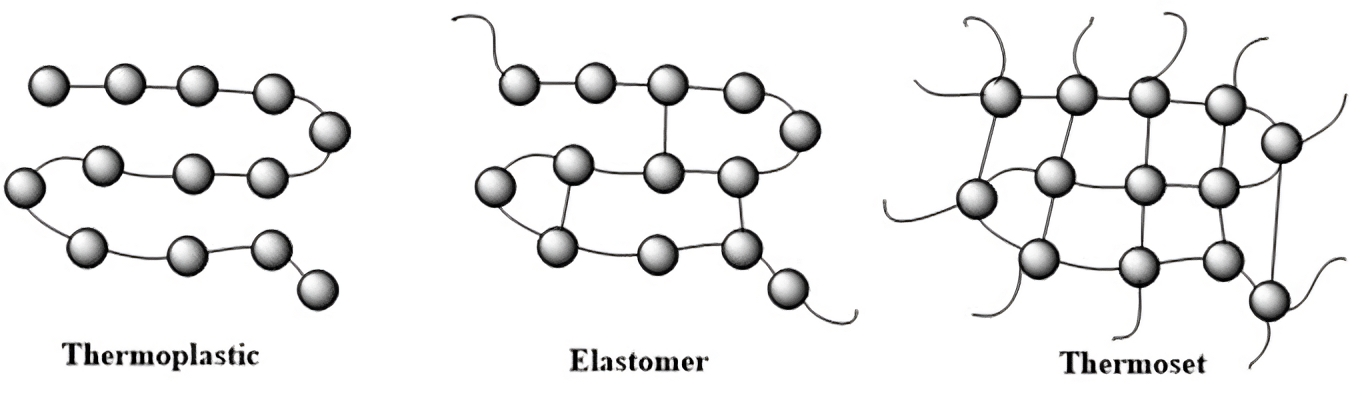
\includegraphics[width=1.0\linewidth]{imgs/elastomer.png}
    \caption{Estructura molecular en distintos tipos de polímeros.}
    \label{plmrs}
\end{figure}

\begin{table}[h]
  \centering
  \caption{Etapas generales en la producción de polímeros}
  \label{tab:etapas_polimeros}
  \begin{tabular}{|P{2.5cm}|P{3.5cm}|P{4cm}|P{4.5cm}|}
    \hline
    \textbf{Etapa}            & \textbf{Estado de la mezcla}        & \textbf{Termoplásticos}                                                    & \textbf{Termoestables}                                                        \\ \hline
    Monómeros                 & Líquido o gas                       & Monómeros aislados listos para reaccionar                                   & Monómeros o precursores con múltiples sitios reactivos                         \\ \hline
    Pre polimerización         & Viscosa (oligómeros cortos)         & Formación de cadenas lineales o ramificadas de bajo peso molecular & Formación de resinas líquidas o prepolímeros con grupos funcionales reactivos   \\ \hline
    Polimerización            & Semifundida o fundida               & Crecimiento de cadenas por adición o condensación sin enlaces cruzados       & Reacción simultánea de formación de cadena y reticulación progresiva            \\ \hline
    Moldeo y conformado       & Fundido (\,TP\,), líquido (\,TE\,)  & Moldeo, enfriado y ciclo repetible tras nueva fusión                         & Moldeo inicial (inyección, compresión) seguido de curado irreversible          \\ \hline
    Post-tratamiento y curado & Sólido                              & Opcional: orientación, recocido, mejora de propiedades                      & Curado final para completar la red tridimensional y obtener rigidez permanente  \\ \hline
  \end{tabular}
\end{table}

En ingeniería, aunque los polímeros suelen exhibir una resistencia mecánica inferior a la de metales o cerámicas, compensan esa desventaja con un coste reducido, una gran versatilidad en los procesos de conformado y una elevada resistencia a la corrosión y a agentes químicos.

Los polímeros muestran una marcada dependencia de la temperatura, lo cual puede limitar su rango de servicio pero al mismo tiempo facilita enormemente su conformado (moldeo, extrusión, inyección). Esta sensibilidad térmica se traduce en variaciones drásticas del módulo de elasticidad y acota los rangos operativos prácticos. 

El fenómeno principal que rige el comportamiento mecánico de los polímeros a bajas y medias temperaturas es la \textbf{transición vítrea} (Figura \ref{vitr}). Se trata de un cambio abrupto en la rigidez y en las propiedades viscoelásticas cuando se supera la \textbf{temperatura de transición vítrea} (\(T_{g}\)). 

Por debajo de \(T_{g}\), las cadenas poliméricas están \comillas{congeladas} en un estado rígido y frágil, con muy escasa movilidad. Al pasar por \(T_{g}\), se activan movimientos de rotación y traslación local de los segmentos de cadena, dando lugar a un estado gomoso o viscoelástico con mayor capacidad de deformación y absorción de energía. Esta transición se explica por el incremento de la energía térmica disponible para vencer las barreras conformacionales de los enlaces simples a lo largo de la macromolécula.

La cristalinidad de un polímero determina sus propiedades térmicas, mecánicas y ópticas. Según el grado de ordenamiento de las cadenas, se pueden distinguir dos grandes familias:

\begin{itemize}
  \item \textbf{Semicristalino:} combinan regiones cristalinas ordenadas (cristalitas) con zonas amorfas. Exhiben un punto de fusión (\(T_m\)) correspondiente a desorganización de las porciones cristalinas y un \(T_g\) asociado a las zonas amorfas. La presencia de cristalinidad aporta mayor rigidez, resistencia química y mejor barrera a gases. Ejemplos típicos: polietileno (PE), polipropileno (PP) y tereftalato de polietileno (PET).
  \item \textbf{Amorfo:} las cadenas carecen de orden a largo alcance y presentan únicamente una temperatura de transición vítrea (\(T_g\)). No existe un punto de fusión bien definido, por lo que mantienen transparencia y flexibilidad a temperatura ambiente. Ejemplos típicos: poliestireno (PS), poli(metacrilato de metilo) (PMMA) y policarbonato (PC).
\end{itemize}

\begin{figure}[h!]
    \centering
    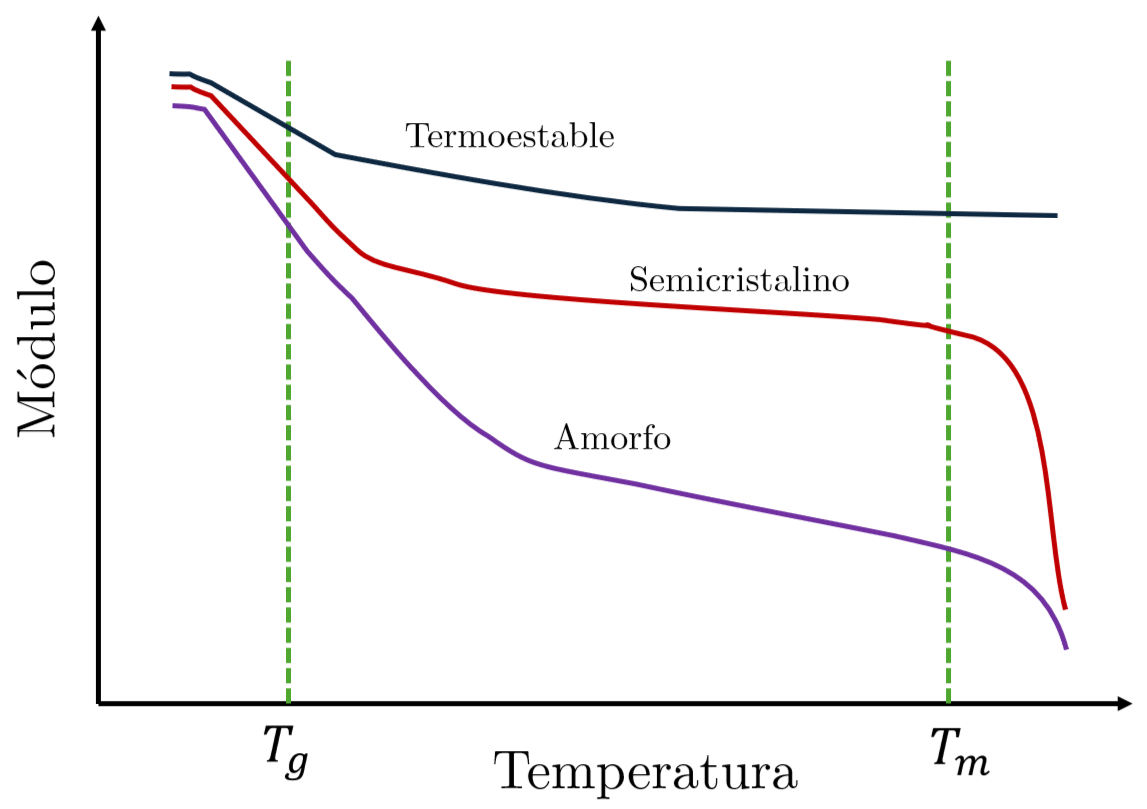
\includegraphics[width=0.8\linewidth]{imgs/tgap.png}
    \caption{Cambio de rigidez con la temperatura en polímeros. La primera línea vertical punteada es la de transición vítrea, la segunda la de fundición.}
    \label{vitr}
\end{figure}

No es posible alcanzar cristalinidad total en polímeros porque sus largas cadenas presentan irregularidades (extremos libres, ramificaciones y defectos) que impiden el empaquetamiento ordenado a lo largo de toda la macromolécula. Además, los entrelazamientos moleculares generan zonas amorfas donde las cadenas no pueden reordenarse en redes cristalinas. Como resultado, siempre coexisten regiones rígidas y ordenadas con áreas desordenadas. En general, los termoestables serán amorfos, pues los enlaces curzados limita el ordenamiento regular de las cadeas.

En los polímeros semicristalinos, el nivel de cristalinidad (habitualmente un 30–70$\%$) influye en la densidad, la tenacidad y la barrera al vapor de agua. Por el contrario, los amorfos suelen presentar una amplia ventana térmica de procesado, lo que facilita operaciones como moldeo por inyección o extrusión.

Cuando un polímero se somete a esfuerzo mecánico, su deformación avanza en varias etapas (Figura \ref{plastens}). Estas dependerán del grado de reticulación (enlaces cruzados) pues limitarán el movimiento de las cadenas, definiendo en parte la ductilidad o fragilidad de un material.

Región elástica: en esta fase inicial la curva esfuerzo–deformación es prácticamente lineal y reversible. Las cadenas poliméricas no se estiran como resortes, sino que giran alrededor de sus enlaces y se reajustan conformacionalmente. Al retirar la carga, la entropía y las rotaciones de enlace devuelven al polímero a su forma original.

Límite de fluencia: al superar el esfuerzo lineal máximo, la curva se aplanará o caerá ligeramente. Aquí las cadenas amorfas empiezan a deslizarse unas sobre otras y se inicia la deformación plástica. La muestra ya no recupera completamente su forma al descargar.

Deformación plástica y necking inicial: la carga adicional provoca la formación de un cuello en una región localizada. La sección transversal disminuye y las cadenas se reorientan alineándose con la dirección de tracción. El esfuerzo se mantiene alrededor de un valor medio mientras avanza el estrechameiento.

Endurecimiento por orientación molecular: tras el necking, la contínua alineación de las cadenas genera un aumento de rigidez. El esfuerzo vuelve a ascender porque las macromoléculas orientadas resisten mejor la carga, exhibiendo un refuerzo mecánico visible en la curva.

Estrechamiento final y fractura: la estricción se concentra hasta que la sección remanente ya no soporta más carga. Se produce una caída brusca del esfuerzo y ocurre la rotura. En polímeros dúctiles la superficie de fractura presenta fibrillas o regiones estiradas.


\begin{figure}[h!]
    \centering
    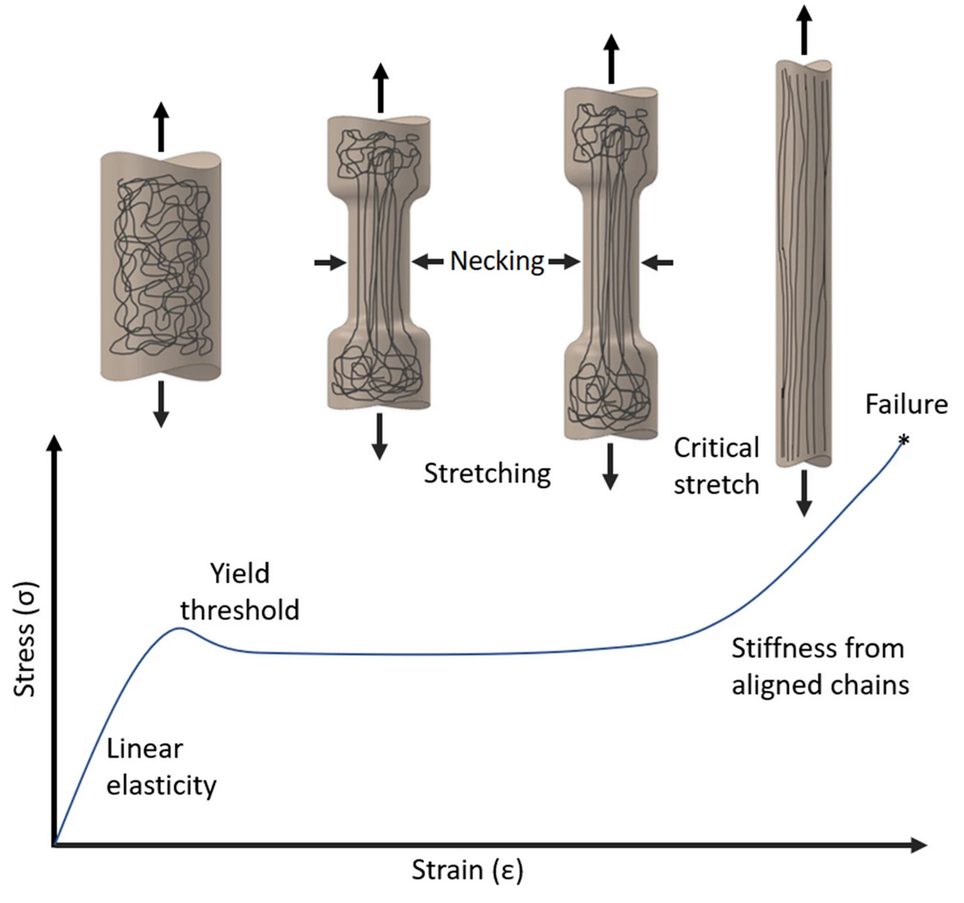
\includegraphics[width=0.8\linewidth]{imgs/estre.png}
    \caption{Curva de esfuerzo-deformación para un polímero dúctil.}
    \label{plastens}
\end{figure}

Un caso particular de comportamiento mecánico es el de los elastómeros. Sus macromoléculas carecen de orden a largo alcance gracias a su microestructura atáctica, en la que los grupos laterales se disponen de modo aleatorio. Esta disposición impide la formación de cristales y mantiene al polímero en un estado amorfo, donde las cadenas pueden adoptar un gran número de conformaciones distintas sin quedar atrapadas en una red ordenada.

La presencia de enlaces dobles en configuración cis introduce \comillas{kinks} (curvatura local) o doblamientos en la columna vertebral de la cadena, aumentando aún más la variedad de conformaciones accesibles. Cada kink favorece que las cadenas no se alineen y, por tanto, que no cristalizen; esto multiplica el número de microestados posibles y amplía la capacidad de deformación reversible.

Para que esa libertad conformacional derive en un comportamiento elástico, las cadenas se interconectan mediante una red de enlaces cruzados de baja densidad. Los entrecruzamientos actúan como puntos de anclaje que fijan la longitud máxima de cada cadena: evitan el flujo plástico, pero al mismo tiempo permiten el desenredo y replegado de segmentos bajo tensión.

Cuando se aplica una fuerza, el elastómero se estira reduciendo drásticamente el número de conformaciones posibles (disminuye la entropía). Al descargarse, la impulsión termodinámica busca restaurar el máximo desorden, de modo que las cadenas regresan casi por completo a su configuración inicial. Este mecanismo puramente entrópico es el origen de la alta elasticidad y de la recuperación casi total de la forma original en los elastómeros. 

Un fenómeno curioso se da cuando un elastómero estirado se calienta por encima de su temperatura ambiente, la energía térmica adicional aumenta la movilidad de segmentos en las cadenas de la red reticulada. Sin embargo, en lugar de expandirse, el material se contrae: al elevar la temperatura se refuerza el impulso entrópico que tiende a maximizar el número de conformaciones posibles de cada cadena. Debido a los enlaces cruzados, las macromoléculas no pueden deslizarse unas sobre otras, por lo que el único modo de recuperar el máximo desorden es acortando la distancia entre puntos de reticulación. Este efecto se denomina retracción térmica o efecto termoelástico.

Los polímeros suelen presentar una alta absorción de humedad o \textbf{higroscopicidad} respecto a otros materiales de ingeniería, debido a la presencia de grupos funcionales polares (hidroxilos, ésteres, amidas) en sus cadenas moleculares que establecen enlaces de hidrógeno con el agua.  



Esta captación de humedad impacta negativamente en sus propiedades mecánicas (Figura \ref{humid})porque las moléculas de agua actúan como plastificantes: aumentan la movilidad de las cadenas poliméricas, reducen el módulo de elasticidad y la resistencia a la tracción, y pueden favorecer la hidrólisis de enlaces, generando microfisuras. Como resultado, se degradan la tenacidad, la estabilidad dimensional y la durabilidad de las piezas.

\begin{figure}[h!]
    \centering
    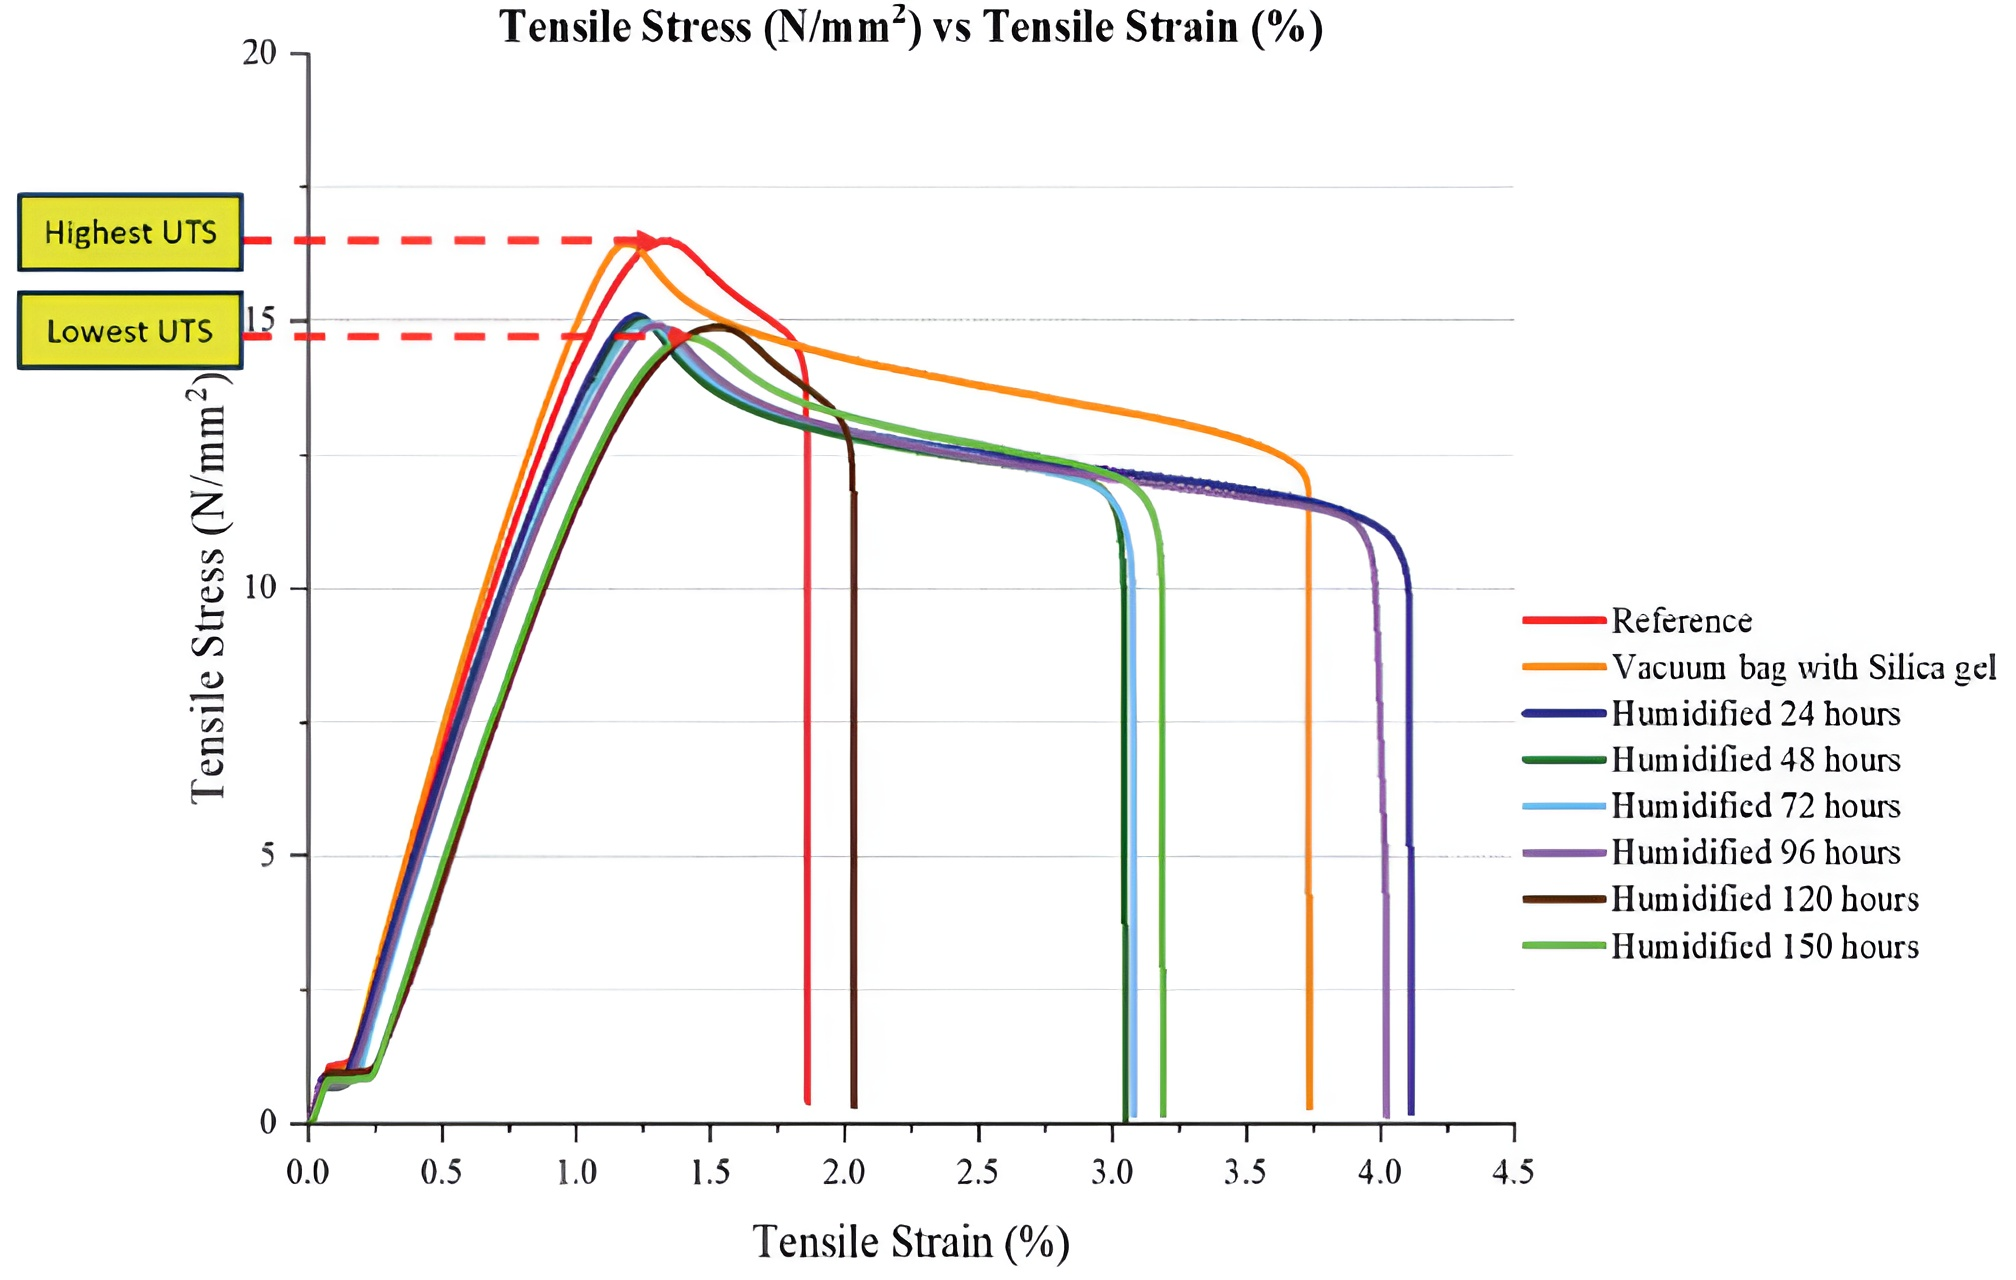
\includegraphics[width=1.0\linewidth]{imgs/humd.png}
    \caption{Gráfico de esfuerzo deformación para un polímero en distintas condiciones de humectación.}
    \label{humid}
\end{figure}